\documentclass[12pt]{article}
\usepackage[spanish]{babel}
\usepackage[utf8]{inputenc}
\usepackage{amsmath}
\usepackage{graphicx}
\usepackage{geometry}
\usepackage{float}
\usepackage{hyperref}
\geometry{margin=2.5cm}

\title{Proyecto No. 1 \\ Máquina de Turing para Fibonacci \\ (Implementación por recurrencia real)}
\author{
Mia Alejandra Fuentes Mérida - 23775 \\
Angel Esteban Esquit Hernández - 23221
}
\date{27 de febrero de 2026}

\begin{document}

\maketitle

\section{Notación Asintótica O (Big-O)}

La notación Big-O describe el límite superior del crecimiento de una función cuando el tamaño de la entrada tiende a infinito.

Formalmente:

\[
f(n) \in O(g(n))
\]

si existen constantes positivas $c$ y $n_0$ tales que:

\[
0 \le f(n) \le c g(n) \quad \forall n \ge n_0
\]

Big-O permite modelar el crecimiento del número de pasos ejecutados por un algoritmo conforme aumenta el tamaño de la entrada.

---

\section{Convenciones de Representación}

\subsection{Representación Unaria}

Se utiliza representación unaria:

\begin{itemize}
\item $0 \rightarrow$ cadena vacía
\item $1 \rightarrow 1$
\item $2 \rightarrow 11$
\item $n \rightarrow 1^n$
\end{itemize}

La entrada consiste en una cadena de $n$ símbolos 1.

\subsection{Alfabetos}

\textbf{Alfabeto de entrada:}

\[
\Sigma = \{1\}
\]

\textbf{Alfabeto de la cinta:}

\[
\Gamma = \{1,\_, |, \#, n, x, a, A, b, B, c\}
\]

Estos símbolos permiten implementar los acumuladores y marcadores necesarios para la recurrencia iterativa.

---

\section{Definición Formal de la Máquina}

La Máquina de Turing se define como la 7-tupla:

\[
M = (Q, \Sigma, \Gamma, \delta, qStart, \_, F)
\]

Donde:

\begin{itemize}
\item $Q$ es el conjunto finito de estados (30 estados).
\item $\Sigma = \{1\}$
\item $\Gamma = \{1,\_, |, \#, n, x, a, A, b, B, c\}$
\item $\delta$ es la función de transición
\item $qStart$ es el estado inicial
\item $F = \{qAccept\}$
\end{itemize}

La función de transición está definida en el archivo \texttt{fib\_tm\_real.json} y contiene 132 transiciones.

---

\section{Idea General del Funcionamiento}

A diferencia de la versión anterior, esta máquina no tiene valores de Fibonacci predefinidos.

Implementa la recurrencia real:

\[
F(n) = F(n-1) + F(n-2)
\]

La estrategia consiste en:

\begin{enumerate}
\item Convertir la entrada $1^n$ en marcadores $n$.
\item Inicializar acumuladores:
\[
a = F(0), \quad b = F(1)
\]
\item Por cada símbolo $n$ restante:
\begin{itemize}
\item Copiar $a$ y $b$ hacia un área temporal
\item Construir $c = a + b$
\item Reasignar:
\[
a \leftarrow b
\]
\[
b \leftarrow c
\]
\end{itemize}
\item Al finalizar, limpiar marcadores y dejar únicamente $b$ en notación unaria.
\end{enumerate}

Esto produce una simulación iterativa real de Fibonacci en una sola cinta.

---

\section{Análisis Empírico}

Se realizaron pruebas para:

\[
n = 0,1,2,\dots,18
\]

Con límite de 50,000,000 pasos.

Para cada ejecución se registró:

\begin{itemize}
\item Pasos ejecutados
\item Tiempo de CPU
\item Estado final
\item Valor leído en cinta
\end{itemize}

Se observó crecimiento acelerado conforme aumenta $n$.

---

\section{Regresión Polinomial}

\subsection{Pasos de ejecución}

Modelo de grado 3:

\[
pasos(n) = 4.64\times10^{4} n^3 - 9.228\times10^{5} n^2 + 4.602\times10^{6} n - 3.813\times10^{6}
\]

\[
R^2 = 0.8605
\]

\subsection{Tiempo de CPU}

Modelo de grado 3:

\[
tiempo(n) = 0.02249 n^3 - 0.4471 n^2 + 2.23 n - 1.848
\]

\[
R^2 = 0.8602
\]

---

\section{Notación Asintótica Experimental}

Empíricamente:

\[
T(n) \in O(n^3)
\]

En el rango evaluado.

---

\section{Gráficas}

\begin{figure}[H]
\centering
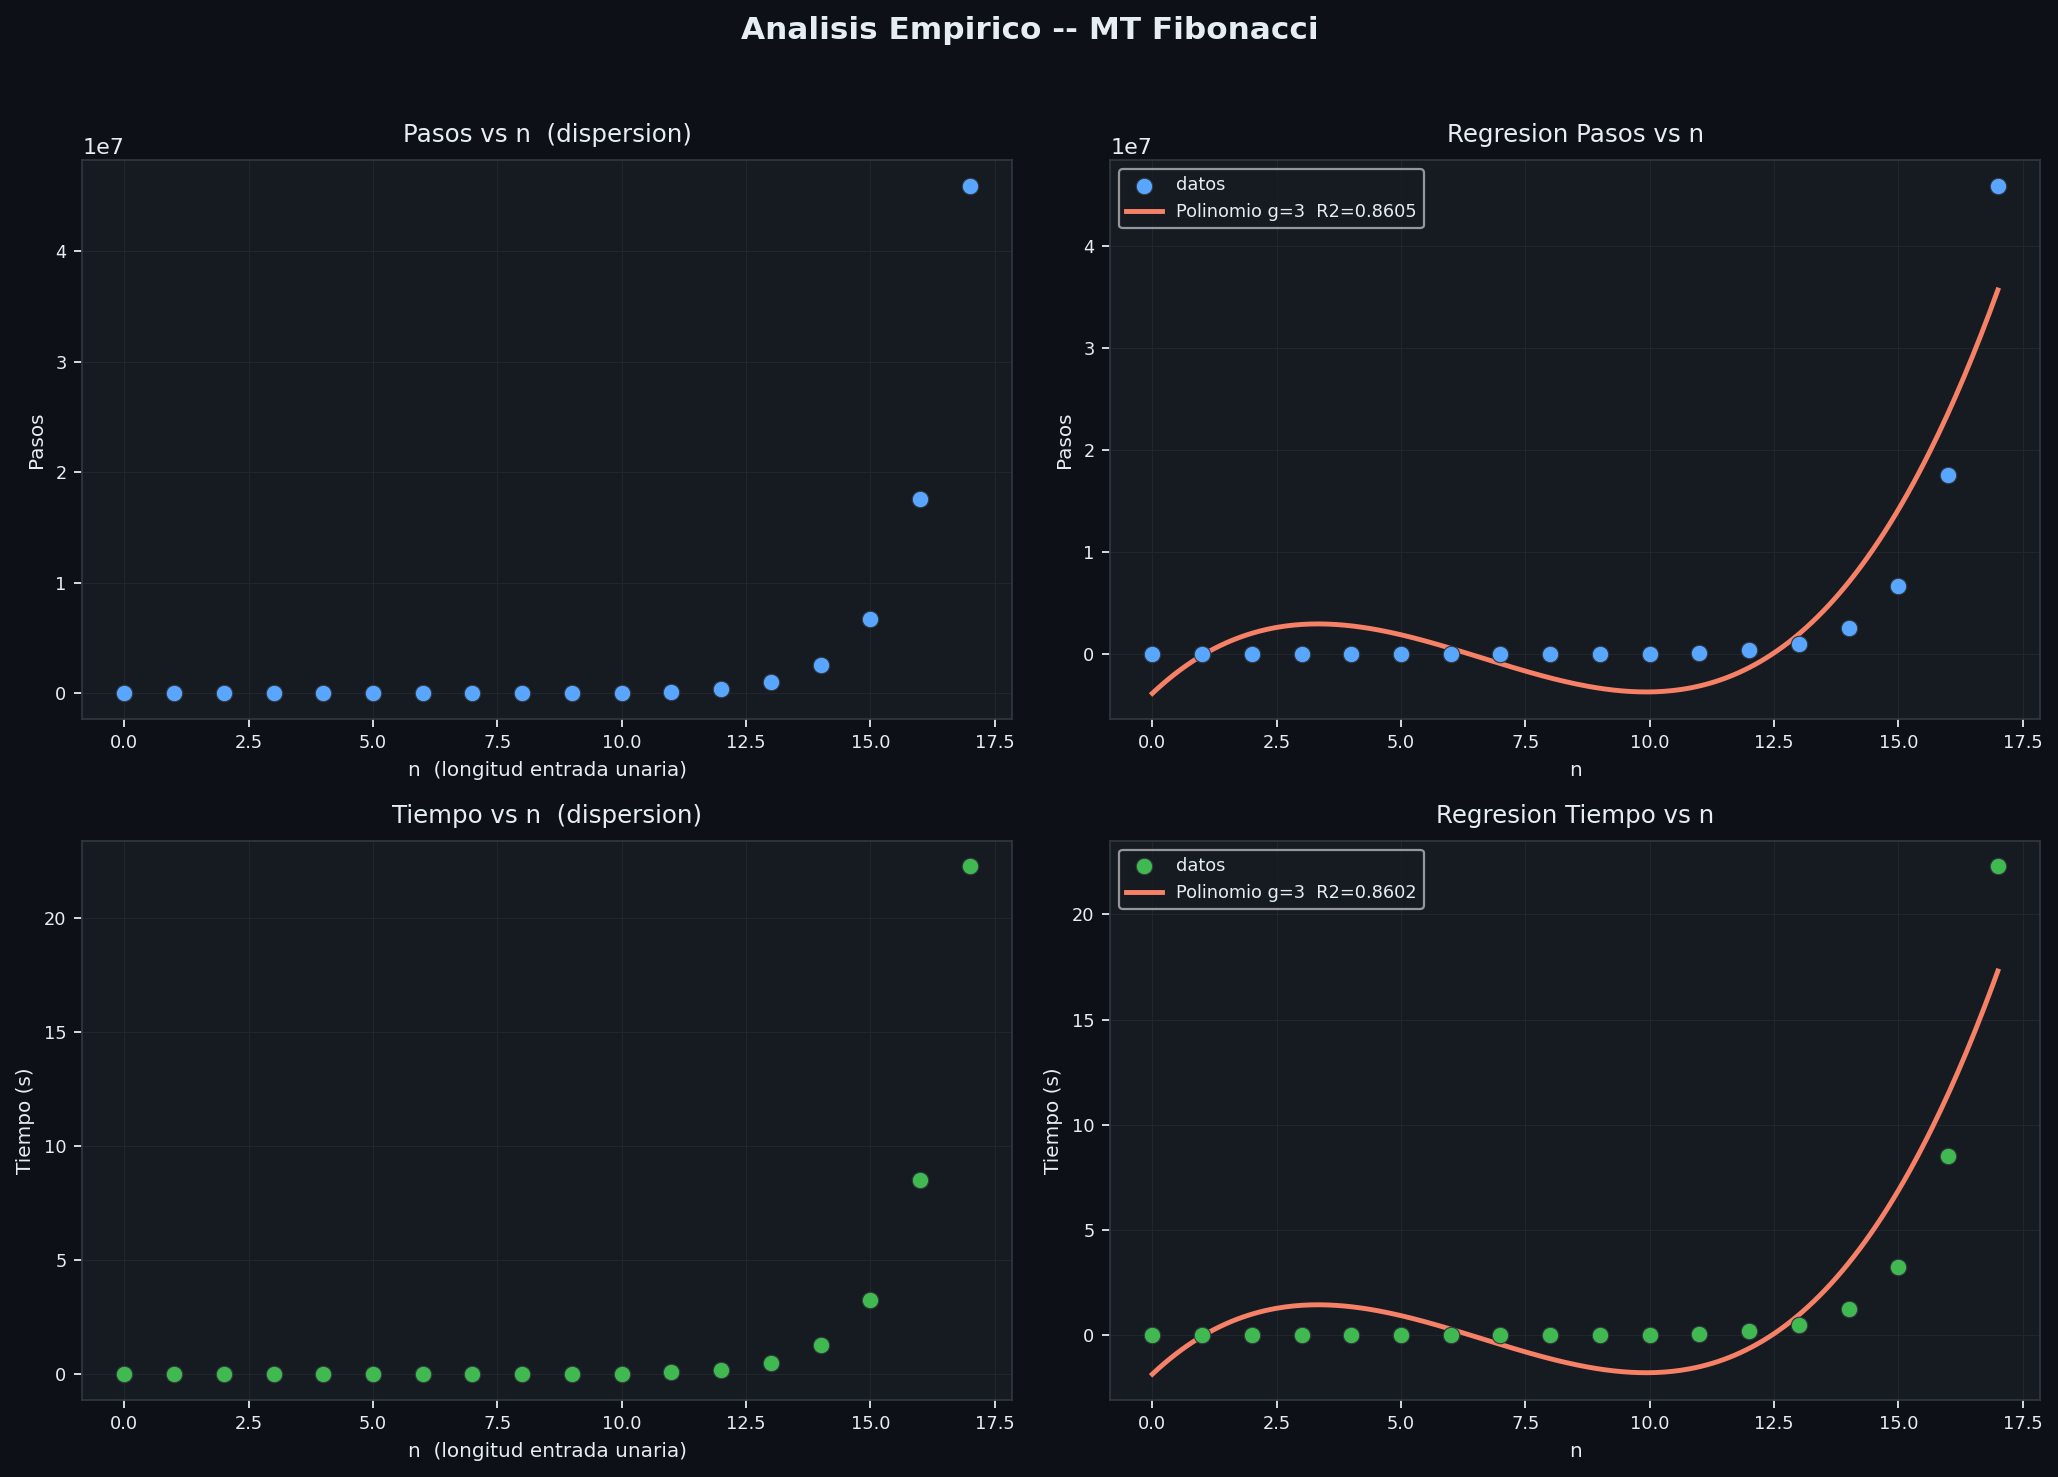
\includegraphics[width=0.9\textwidth]{analisis_tm.png}
\caption{Análisis empírico: pasos y tiempo vs n}
\end{figure}

---

\section{Conclusiones}

La nueva implementación:

\begin{itemize}
\item No hardcodea valores.
\item Implementa recurrencia real.
\item Escala significativamente peor que la versión anterior.
\item Presenta crecimiento cúbico empírico.
\end{itemize}

---

\section{Repositorio}

\url{https://github.com/miafuentes30/Proyecto-1-ADP.git}

\end{document}